\chapter{shadowLB}
\label{related-shadow}

\section{概要}
本研究ではSIIT-DCにおける動的なEAMTの管理・制御手法の実現を目指す.以後このような機構をダイナミックEAMT機構と呼称する.

本章では考えられる手法を大別した上でその特徴と利点及び欠点を挙げ,最も適した手法を検討する.


% \section{求められる要件}
% \label{consideration:points}
% 前で述べたIPv4サービス提供手法の機能要件とSIIT-DCの現状の課題を総括し,EAMTを動的に制御する手法に求められる要件を下記のように定義した.

% \begin{enumerate}
%     \item \textbf{BR間のEAMTの一貫性} \\
%     障害時の適切なフェイルオーバを実現するためには,ネットワーク内の各BRが有するEAMTの一貫性が保証される必要がある.
%     \item \textbf{変更追従性} \\
%     近年のIDCでは多数の物理サーバーを統合的に管理するプライベートクラウド環境やコンテナオーケストレーション環境\footnote{Container Orchestration.コンテナ型仮想化統合管理環境}が普及しており,アプリケーション・サービスの追加及び削除が頻繁に行われている.サービスの障害を検知し,適切に冗長系に移行するための手法として,SLB(Servver Load Balancer)が広く利用されている.SIIT-DCのIPv4サービス提供の場でも,サービスの状態の変動にリニアに対応しフェイルオーバーできるような働きが求められる.
%     \item \textbf{スケーラビリティ} \\ 
%     IPv6シングルスタックネットワークにおけるIPv4サービスの提供では水平スケールが容易に行える仕組みを備える必要がある.IPv4サービスを行うサーバの増設や,対外接続点が増えた場合のBRの拡大に十分に適用するスケーラビリティを有することが望ましい.
%     \item \textbf{デプロイメントの容易さ} \\ 
%     SIIT-DCの最も特筆すべきメリットの一つにデプロイメントの容易さが挙げられる.これを損なうことくダイナミックEAMTを実現する必要がある.
% \end{enumerate}


% \section{アプローチの分類と比較}
% \label{consideration:approach}
% はダイナミックEAMTを実現するアプローチとして,二つのアプローチを考察する.それぞれのアプローチで考えられる実装と実際の構成,及び第\ref{consideration:points}節で述べた各要件への適合性を定性的に評価する.

% 本節ではスケーラビリティの評価のために,制御に必要な通信コネクション数による比較を行う.以後BRの数を$M$,IPv4サービスを提供するサーバの数を$N$とし,総通信コネクション数を$C$として表現する.



% \subsection{中央管理型アプローチ}
% \label{consideration:approach:centerized}

% \begin{figure}[h]
%     \begin{center}
%       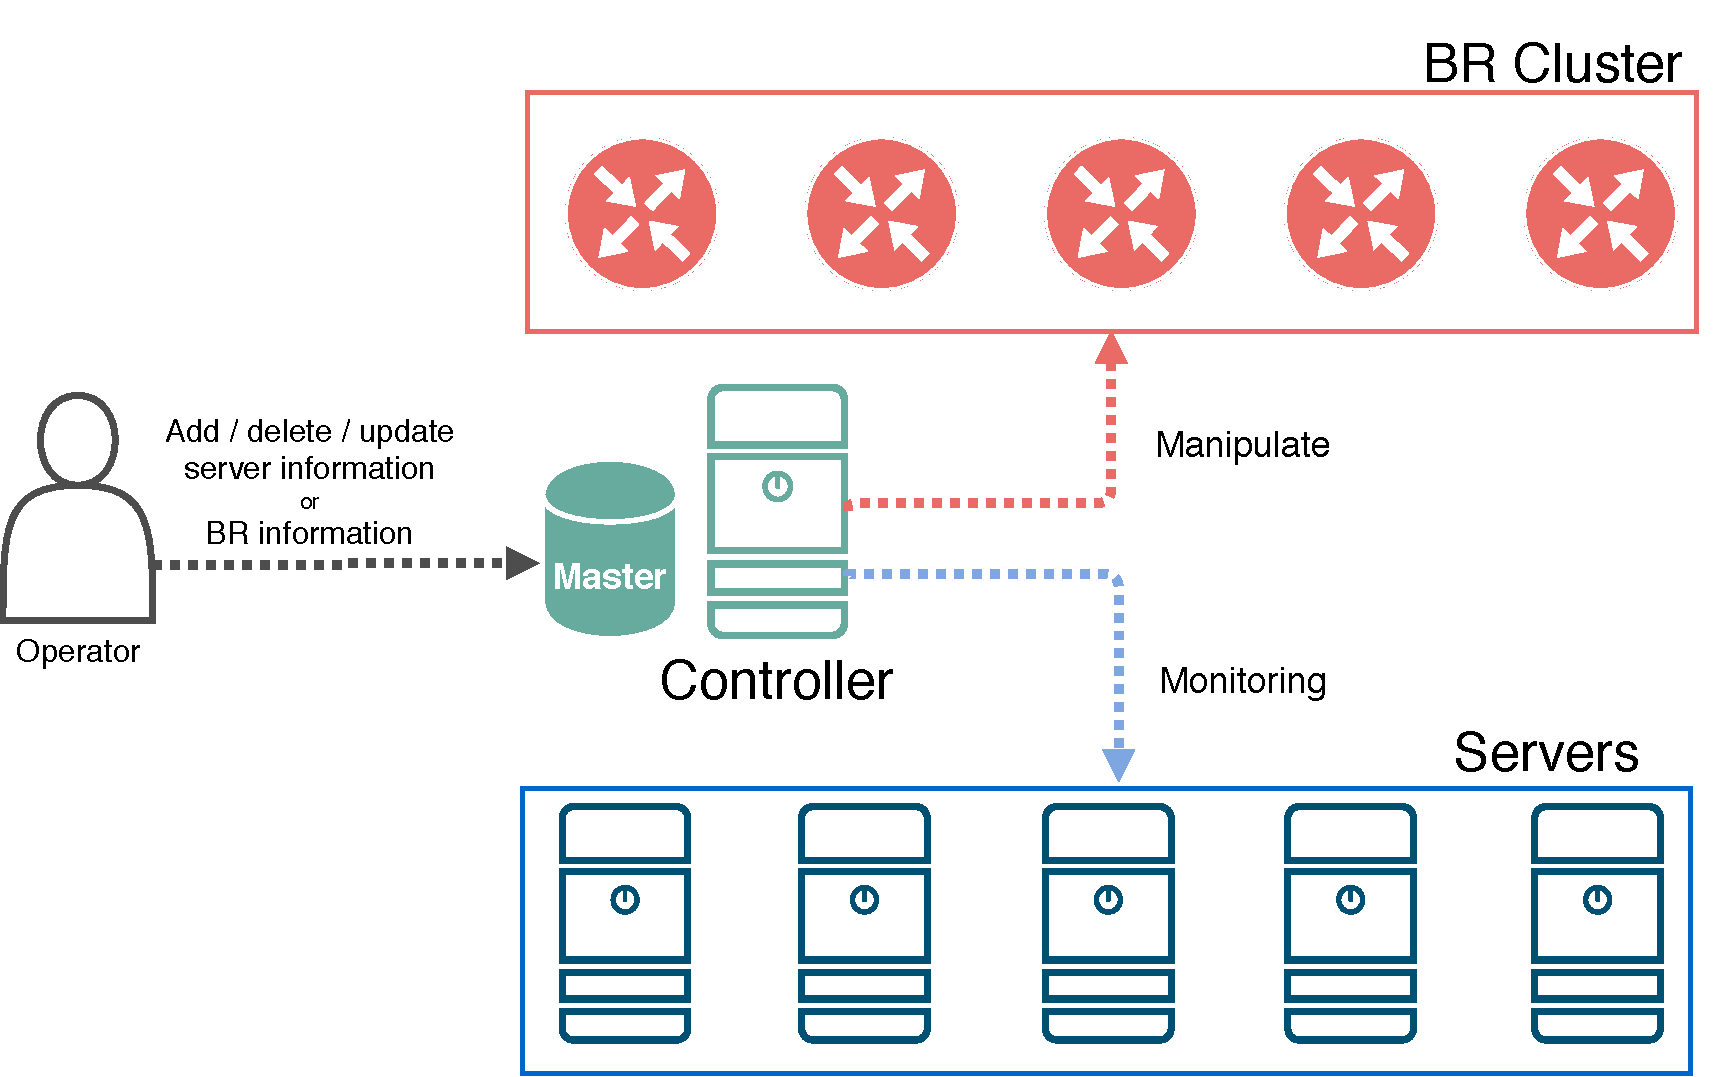
\includegraphics[width=12cm,pagebox=cropbox,clip]{img/approach_centerized_model.pdf}
%     \end{center}
%     \caption{中央管理型アプローチによるダイナミックEAMT}
%     \label{fig:approach_centerized_model}
% \end{figure}

% 中央管理型アプローチとは,複数のBRのEAMTを統合的に管理する「コントローラ」をIDCネットワーク上に配置し,各BRがネットワークを介してこれを参照する機構である.
% 図\ref{fig:approach_centerized_model}に中央管理型アプローチによってダイナミックEAMTを実現したSIIT-DCの各コンポーネントの関係図を示す.

% 中央管理型アプローチではコントローラが各BRに投入するEAMが記録された「マスターテーブル」を保持し,それを元に各BRのデータプレーンにルールを書き込む手法を取る.マスターテーブルに記載されるEAMはオペレーターがネットワークの構成変更に合わせて追加・削除・更新を行い,それぞれのIPv4サービスを提供するサーバ群に対してはコントローラからプル型\footnote{pull-based monitoring. コントローラから各サーバに能動的に情報を取得する}の外部監視\footnote{External monitoring.監視対象でエージェントを稼働することなく,外部から得られる情報を利用して監視を行うこと.}によりサーバの状態変化を検知しマスターテーブルを更新する.

% 本アプローチの実装手法としては,OpenFlow\footnote{Open Networking Foundationにより標準化されているデータプレーン制御用通信プロトコル.\url{https://www.opennetworking.org/}}などを用いた集中コントローラ型SDNフレームワークを利用する方法が考えられる\cite{RFC7426}.類似事例として,ShengらによってOpen Flowを利用して各アクセススイッチにIPv4/IPv6トランスレーション機構をデータプレーンとして導入するデータセンターネットワークデザインの提案がなされている\cite{7560347}.


% \subsubsection{要件評価}

% \begin{itemize}
%     \item BR間のEAMTの一貫性 \\
%     本アプローチでは各BRのEAMTが一つのマスターテーブルからレプリケーションされるために,十分な一貫性が保証される.
%     \item 変更追従性 \\
%     基本的にはEAM情報の更新はオペレーターのマスターテーブルへの記入までの時間はコントローラのサーバ監視性能に依存する.
%     \item スケーラビリティ \\
%     コントローラの数を$L$とすると,EAMTの制御に必要とする総通信コネクション数$C$は以下の通りになる.
%     \begin{equation}
%         C = L(M + N)
%     \end{equation}
%     一方,変更追従性と同じく,管理対象のサーバの収容台数に関しては,コントローラの実装・性能がボトルネックとなる設計である.
%     \item デプロイメントの容易さ \\
%     コントローラに求められる機器の性能・機能要件が大きいため,標準的なSIIT-DCよりデプロイメントのコストは高い.

% \end{itemize}



% \subsection{分散管理型アプローチ}
% 分散管理型アプローチとは,IPv4サービスを提供するサーバがエージェントプロセスを介して自身のIPv4サービスアドレスとIPv6サービスアドレスを広告し,その広告情報を受け取ったBRが自身のEAMTに反映させる機構である.
% 図\ref{fig:approach_distributed_model}に中央管理型アプローチによってダイナミックEAMTを実現したSIIT-DCの各コンポーネントの関係図を表す.

% サーバ群は各BRとEAMを広告するためのコネクションを確立する.IPv4サービスを提供するサーバとBRの間のIPネットワークが何らかの原因により疎通不能になると,当該サーバの広告も同時に停止されるため,該当BRのEAMTから該当するEAMのレコードが削除される.



% \begin{figure}[h]
%     \begin{center}
%       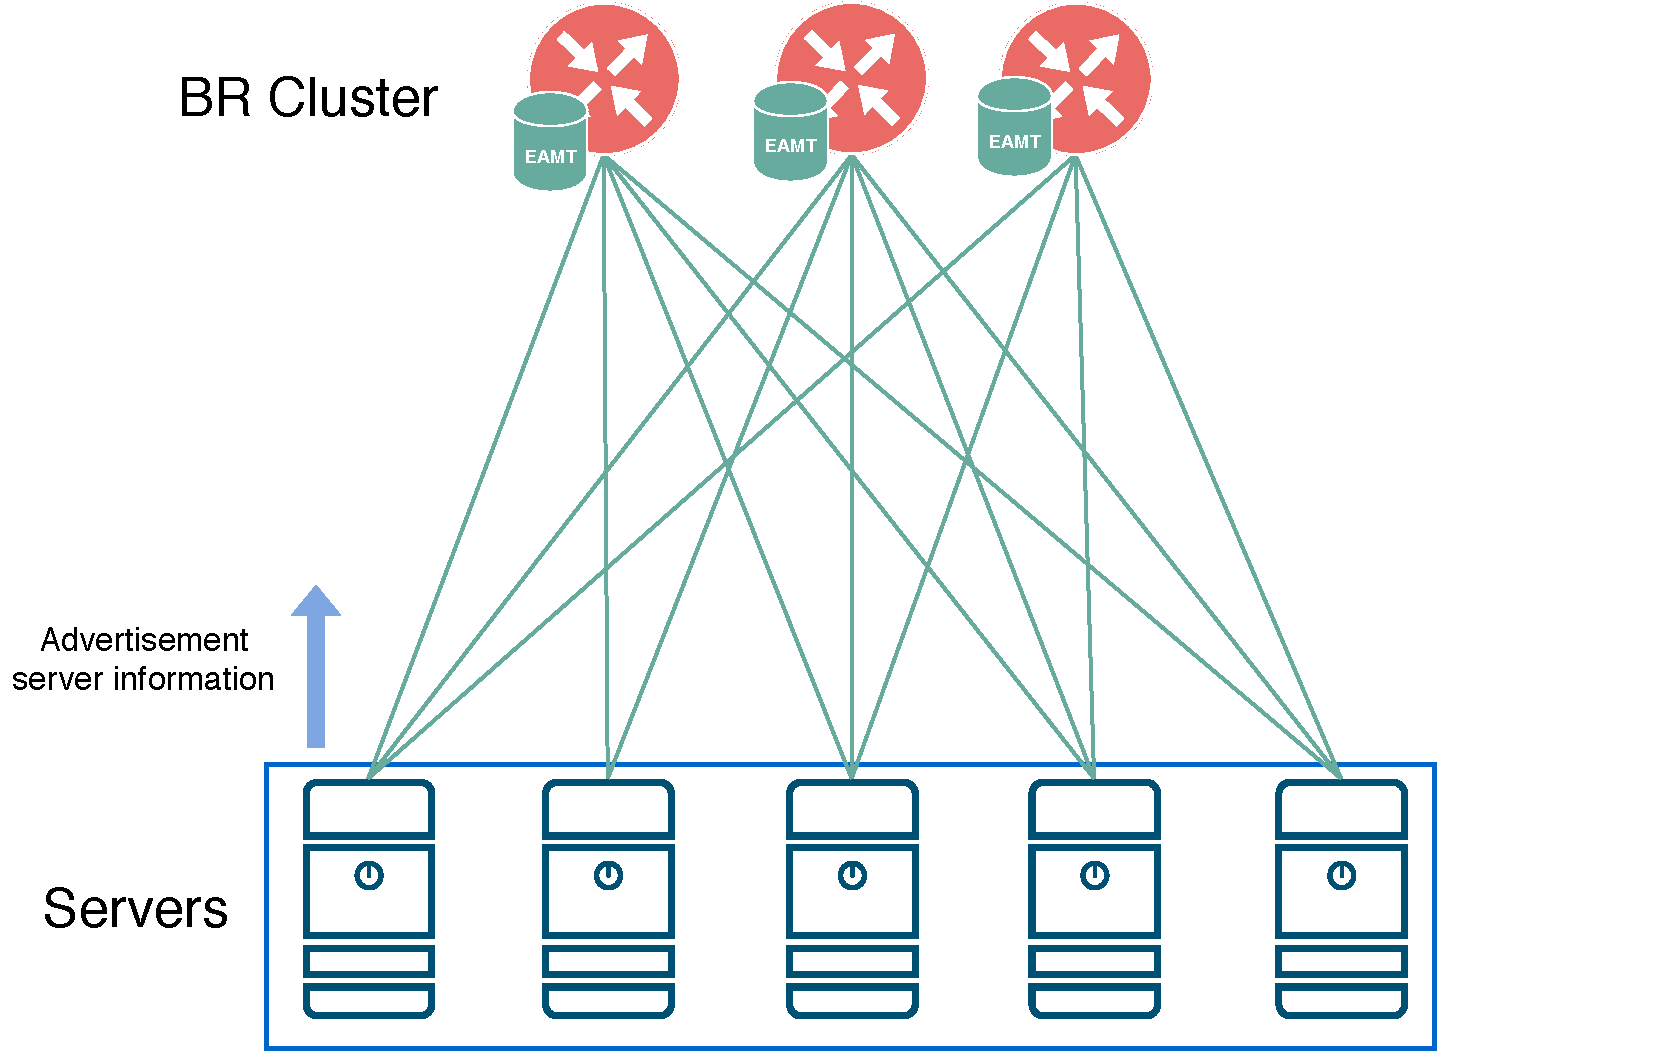
\includegraphics[width=12cm,pagebox=cropbox,clip]{img/approach_distributed_model.pdf}
%     \end{center}
%     \caption{分散管理型アプローチによるダイナミックEAMT}
%     \label{fig:approach_distributed_model}
% \end{figure}

% \subsubsection{要件評価}

% \begin{itemize}
%     \item BR間のEAMTの一貫性 \\
%     各BR間でEAMTの一貫性を保証する機構は無いが,当該BRと疎通できないサーバは障害時に自身のIPv4サービスアドレス宛のトラフィックを当該BRに経由させることが出来ないため,問題にならない.
%     \item 変更追従性 \\
%     サーバ自身のエージェントプロセスが直接BRに広告を行うため,実際の変更にリニアに対応出来る.
%     \item スケーラビリティ \\
%     EAMTの制御に必要とする通信コネクション数$C$は以下の通りになる.
%     \begin{equation}
%         C =  M \cdot N 
%     \end{equation}
%     サーバ群・各BR間でフルメッシュでのコネクションが必要なため,SIIT-DCネットワーク自体が小規模の場合のみ採用可能である.

%     \item デプロイメントの容易さ \\
%     各サーバ・BRにエージェントを導入する必要があるが,システム自体の機能は軽量である.
% \end{itemize}

% \section{アプローチの検討}
% \label{consideration:summary}

% \begin{table}[h]
%     \caption{各アプローチの比較}
%     \label{table:compare_approach}
%     \centering
%     \resizebox{\textwidth}{!}{%
%     \begin{tabular}{lcccc}
%     \hline
%     手法 & EAMTの一貫性 & 変更追従性 & コネクション数 & デプロイメントの容易さ \\ \hline
%     オペレーターによる手動設定 & 無し & 無し & ------ & ----- \\
%     中央管理型アプローチ & 有り & \begin{tabular}[c]{@{}c@{}}\\ (監視機構の実装依存)\end{tabular} & $\frac{L(2M + 2N + L - 1)}{2}$ & \begin{tabular}[c]{@{}c@{}}\\ 困難(コントローラーの実装依存)\end{tabular} \\
%     分散管理型アプローチ & 無し & 有り & $M \cdot N$ & 有り \\ \hline
%     \end{tabular}%
%     }
% \end{table}

% 表\ref{table:compare_approach}に\ref{consideration:points}で述べたダイナミックEAMTに求められる要件に関する両アプローチの比較を示す.
% 中央管理型アプローチが各BR間でのEAMTの一貫性,スケーラビリティの二要素で優位であるが,コントローラの役割が非常に大きくなり機能要件が高くなるため,変更追従性とデプロイメントの容易さの面での障壁が高いという問題を抱えている.一方で分散管理型アプローチはシンプルな構成であるためデプロイメントが比較的容易であり変更への追従がリニアであるが,各サーバが通信コネクションを多量に貼らなくてはならない点でスケーラビリティに難がある.


%%% Local Variables:
%%% mode: japanese-latex
%%% TeX-master: "../bthesis"
%%% End: